% Created 2021-08-06 Fri 10:07
% Intended LaTeX compiler: pdflatex
\documentclass[11pt]{article}
\usepackage[utf8]{inputenc}
\usepackage[T1]{fontenc}
\usepackage{graphicx}
\usepackage{grffile}
\usepackage{longtable}
\usepackage{wrapfig}
\usepackage{rotating}
\usepackage[normalem]{ulem}
\usepackage{amsmath}
\usepackage{textcomp}
\usepackage{amssymb}
\usepackage{capt-of}
\usepackage{hyperref}
\author{David Lewis}
\date{\today}
\title{}
\hypersetup{
 pdfauthor={David Lewis},
 pdftitle={},
 pdfkeywords={},
 pdfsubject={},
 pdfcreator={Emacs 28.0.50 (Org mode 9.5)}, 
 pdflang={English}}
\begin{document}

\tableofcontents

\section{Abstract}
\label{sec:org52343fb}
\section{Introduction}
\label{sec:orgb459187}
\section{Methods}
\label{sec:org2e03ff4}
\subsection{RNA-SEQ}
\label{sec:orgc609234}
\subsubsection{Quantification}
\label{sec:org753876c}
The quant files used for the analysis were the ones generated by the Sailfish quantification tool.
Three other tools were used including the salmon tool, but the results from fastQC were similar enough to
warrant the use of sailfish only. The quant tools were run through the Galaxy system.
\subsubsection{DESEQ2 Vs EdgeR}
\label{sec:orge9a89da}
The quant files were run through both the DESEQ2 and EdgeR differential gene expression analyzers.
The genes were selected as significant when the log2 fold change of the genes were \(\pm\) 2 and the p value was < 0.01. The results from DESEQ2 are used for the conclusions of this paper.
\subsection{WGCNA}
\label{sec:orgbb507c5}
\subsection{GO analysis}
\label{sec:org50ae625}
\subsubsection{Blast}
\label{sec:org4a972d3}

\subsubsection{GProfiler}
\label{sec:org650badf}
functional enrichment analysis. The output from Blast is sent to GProfiler. The GProfiler output is sent to revigo.
\subsubsection{Revigo}
\label{sec:org4ff4065}
The R script output of Revigo generates tree-maps of the genes.
\subsubsection{Geneontolyg.org}
\label{sec:org6f660e8}
The ouptut of blast is sent to Geneontology.org
\section{Results}
\label{sec:orgb19913f}
\subsection{Figure 1: methods comparison between EdgeR and Deseq2}
\label{sec:orgb667e92}
This figure compares the expression data that is present in both EdgeR and Deseq2. The P value is small, indicating that EdgeR and Deseq2 have similar results.
\begin{center}
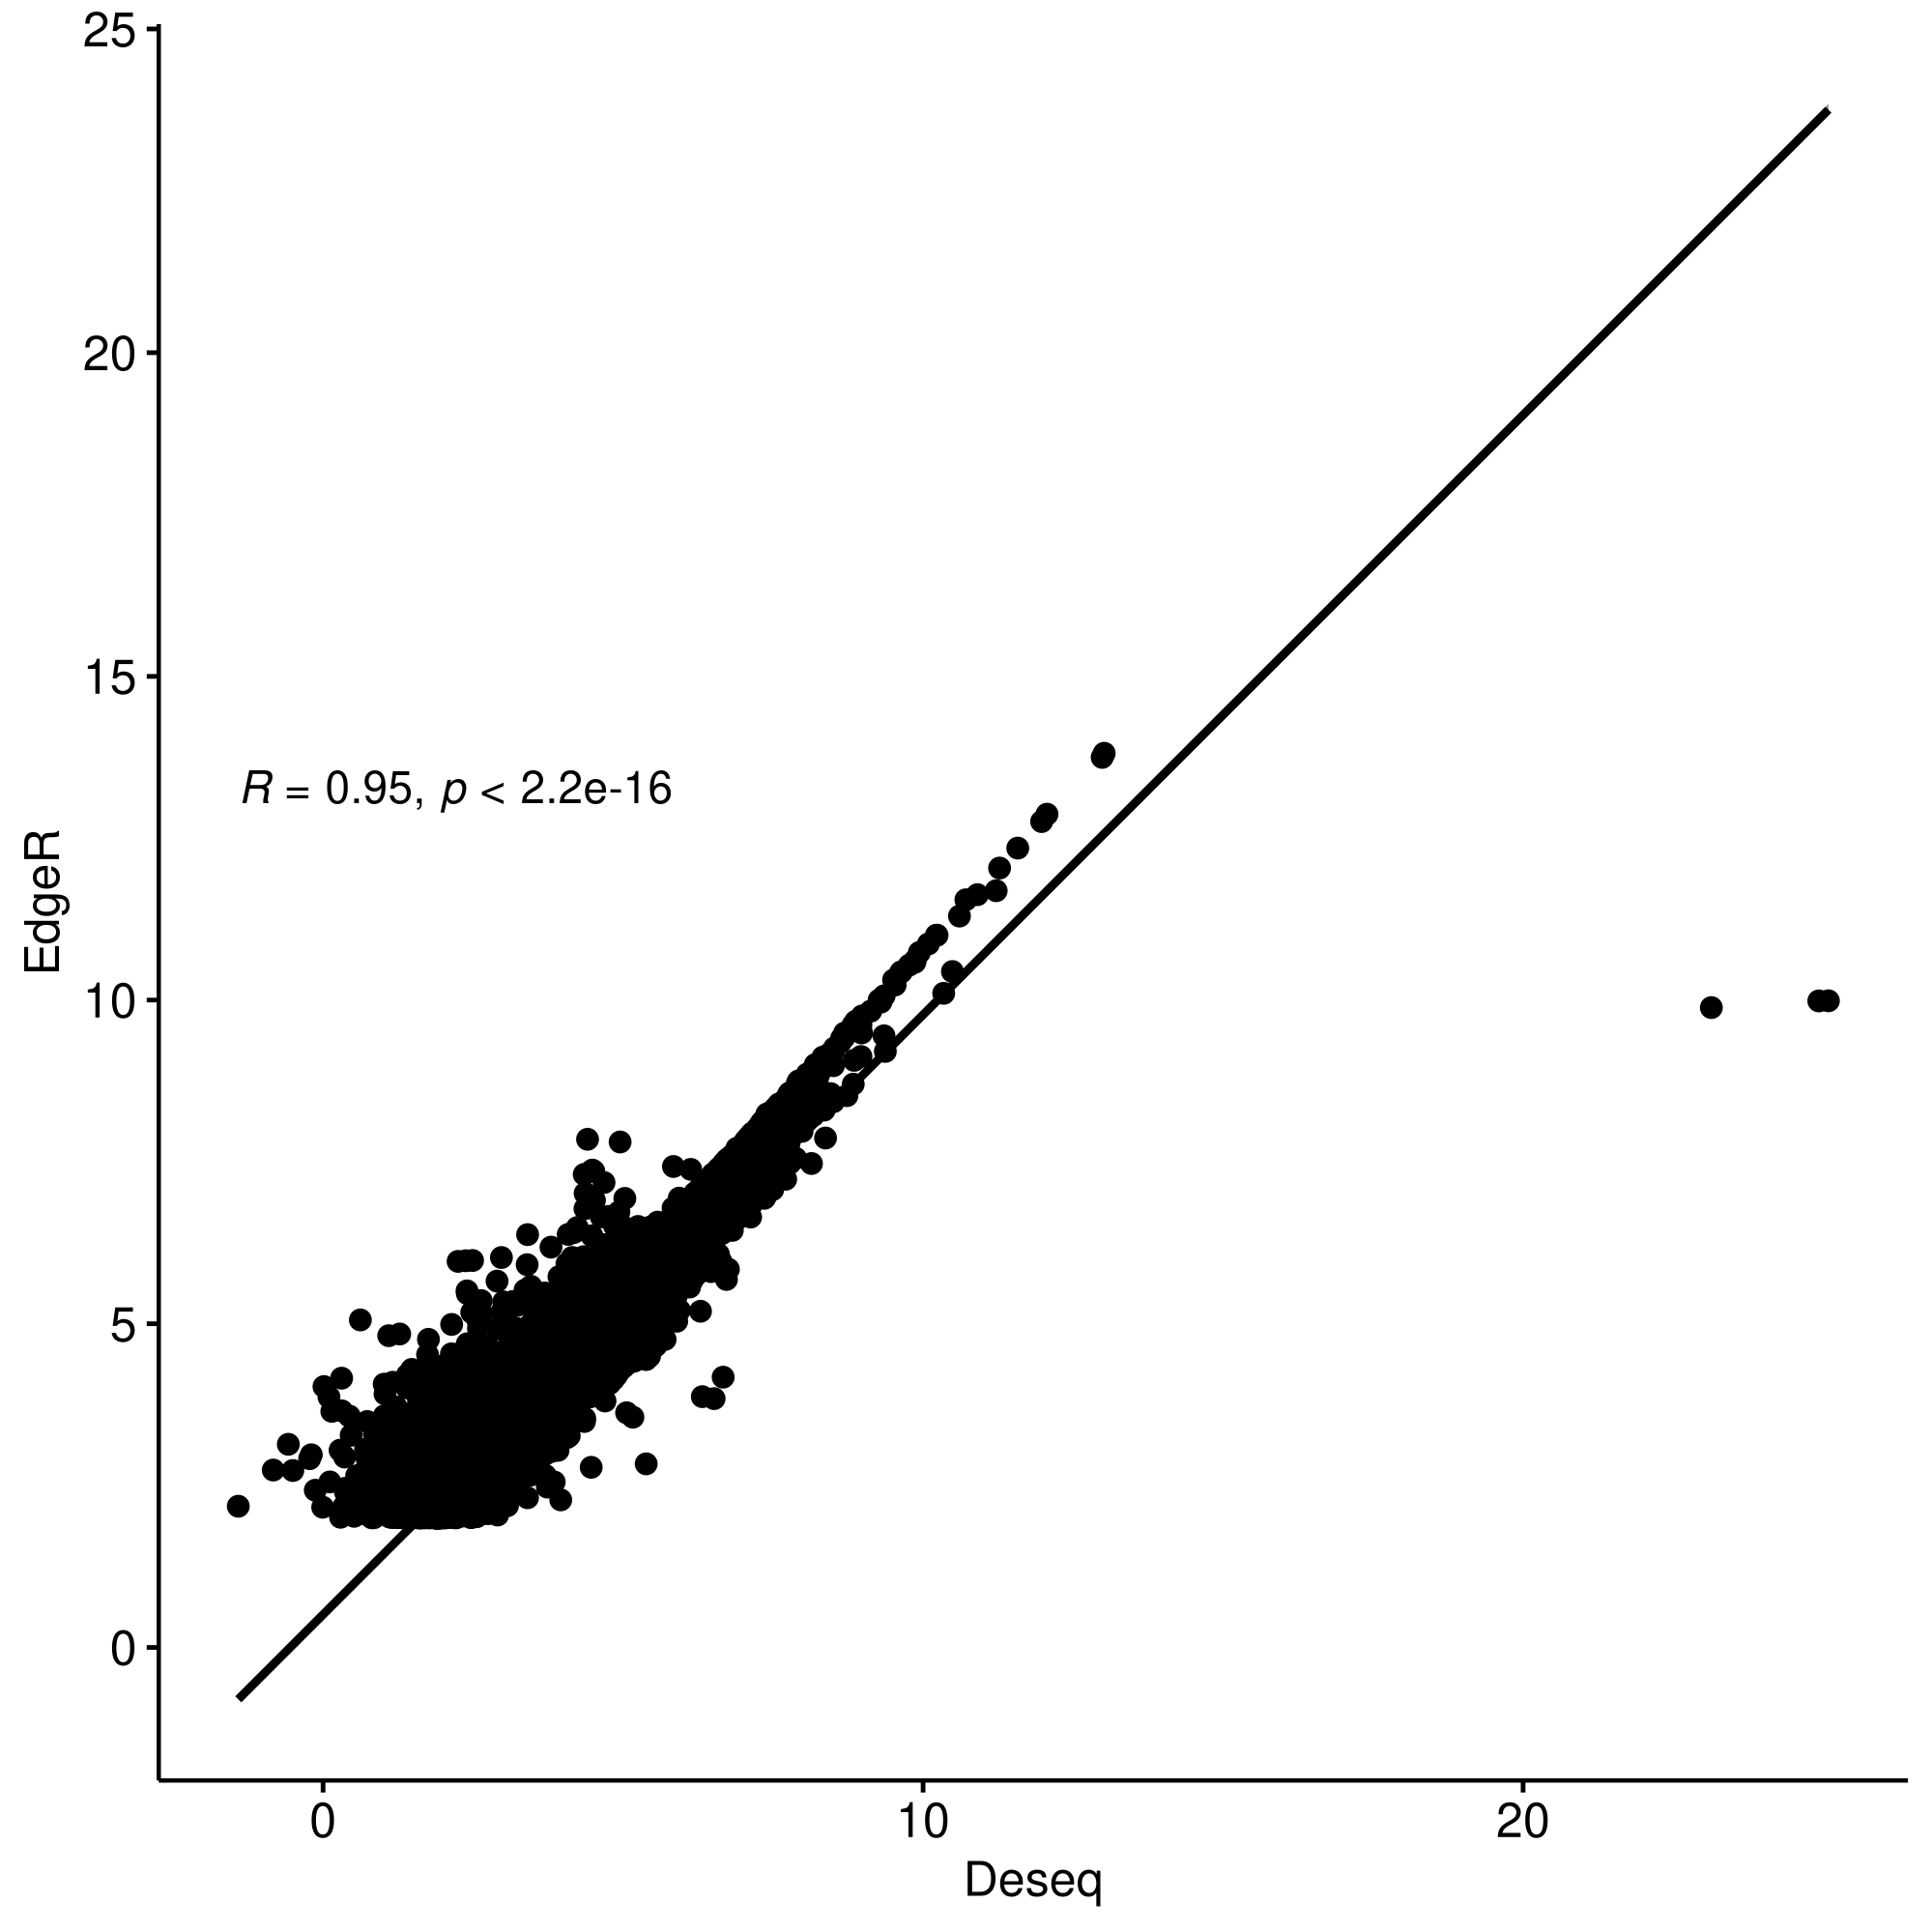
\includegraphics[width=.9\linewidth]{figure1/pearson.png}
\end{center}
\subsection{Figure 2: Perm and Deet repellency and survival}
\label{sec:org526f677}
\subsection{Figure 3: Leg vs Body general (control)}
\label{sec:orgce9bf6f}
This figure compares the genes up-regulated in the body and leg compared to the total number of genes from the sample.
\begin{center}
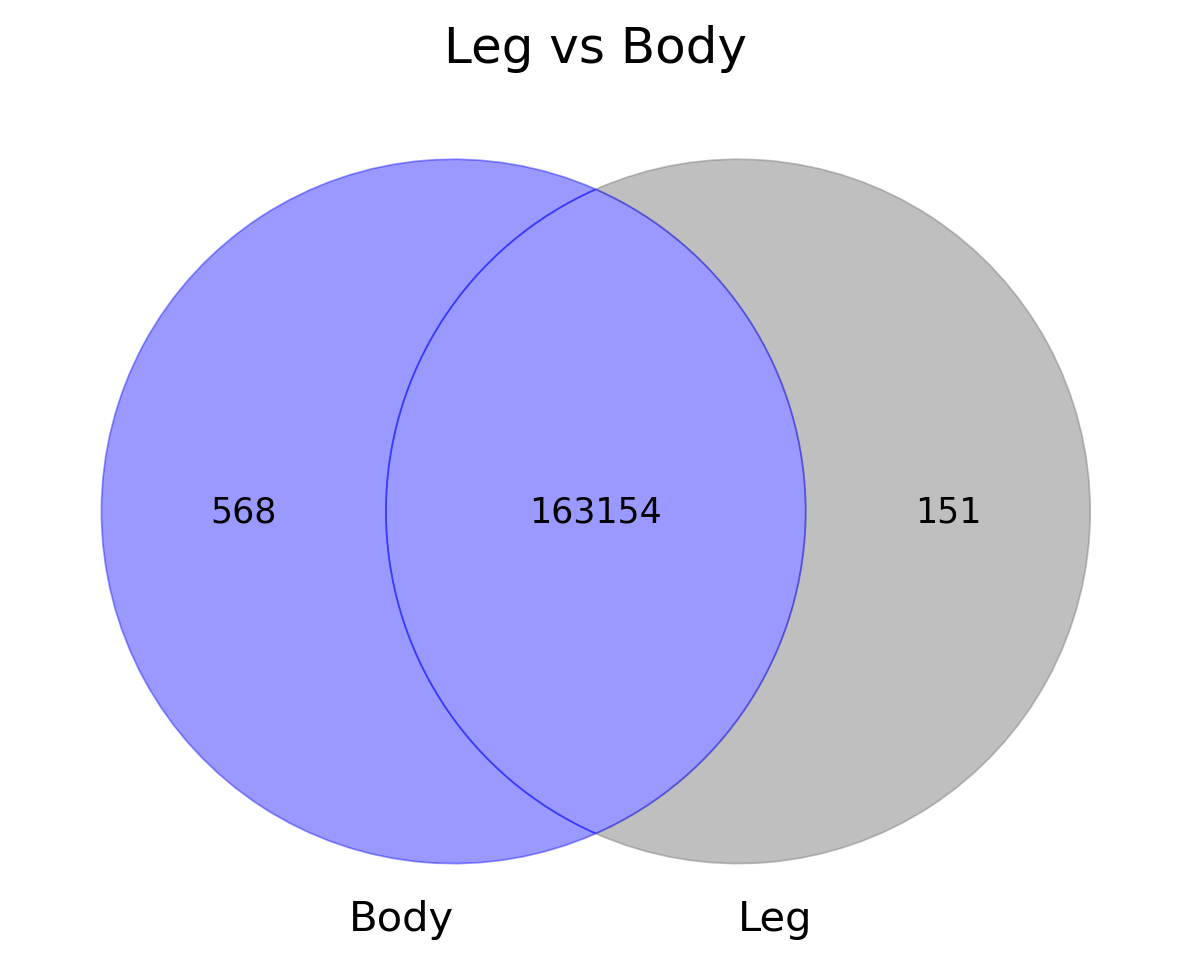
\includegraphics[width=.9\linewidth]{figure3/Deseq-BodyvsLeg.png}
\end{center}
\subsubsection{{\bfseries\sffamily TODO} supplemental tables}
\label{sec:orge417252}
\subsection{Figure 4}
\label{sec:org61576e7}
\subsection{Figure 5:}
\label{sec:orga7443f6}
\subsubsection{Body}
\label{sec:org80b8500}
\begin{center}
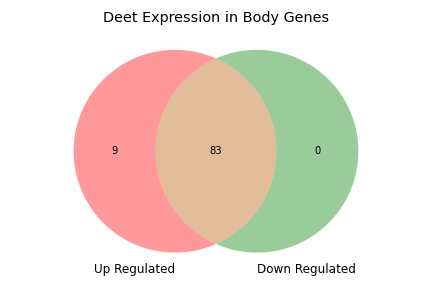
\includegraphics[width=.9\linewidth]{figure5/DeetBodyDeseq.png}
\end{center}
\subsubsection{Leg}
\label{sec:org2f435e9}
\begin{center}
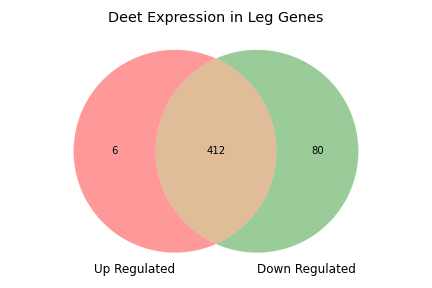
\includegraphics[width=.9\linewidth]{figure5/DeetLegDeseq.png}
\end{center}
\subsubsection{{\bfseries\sffamily TODO} supplemental tables}
\label{sec:orgb78b77b}
\subsection{Figure 6:}
\label{sec:org305e391}
\subsubsection{Body}
\label{sec:orgf38097f}
\begin{center}
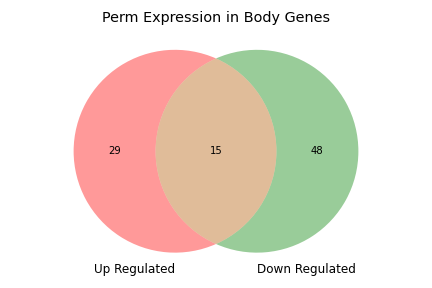
\includegraphics[width=.9\linewidth]{figure6/PermBodyDeseq.png}
\end{center}
\subsubsection{Leg}
\label{sec:orgf9dbc02}
\begin{center}
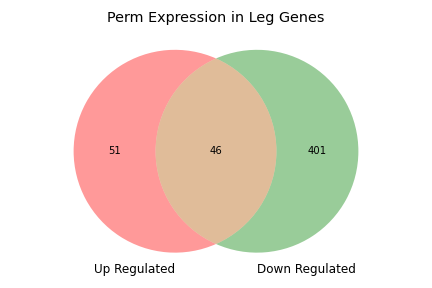
\includegraphics[width=.9\linewidth]{figure6/PermLegDeseq.png}
\end{center}
\subsubsection{{\bfseries\sffamily TODO} supplemental tables}
\label{sec:orgdd49d6b}
\subsection{Figure 7:}
\label{sec:org655fa3a}
\subsection{Figure 8}
\label{sec:org9a76e36}
\subsection{Figure 9:}
\label{sec:org87ea6df}
\subsubsection{DEET}
\label{sec:org81930ab}
\begin{center}
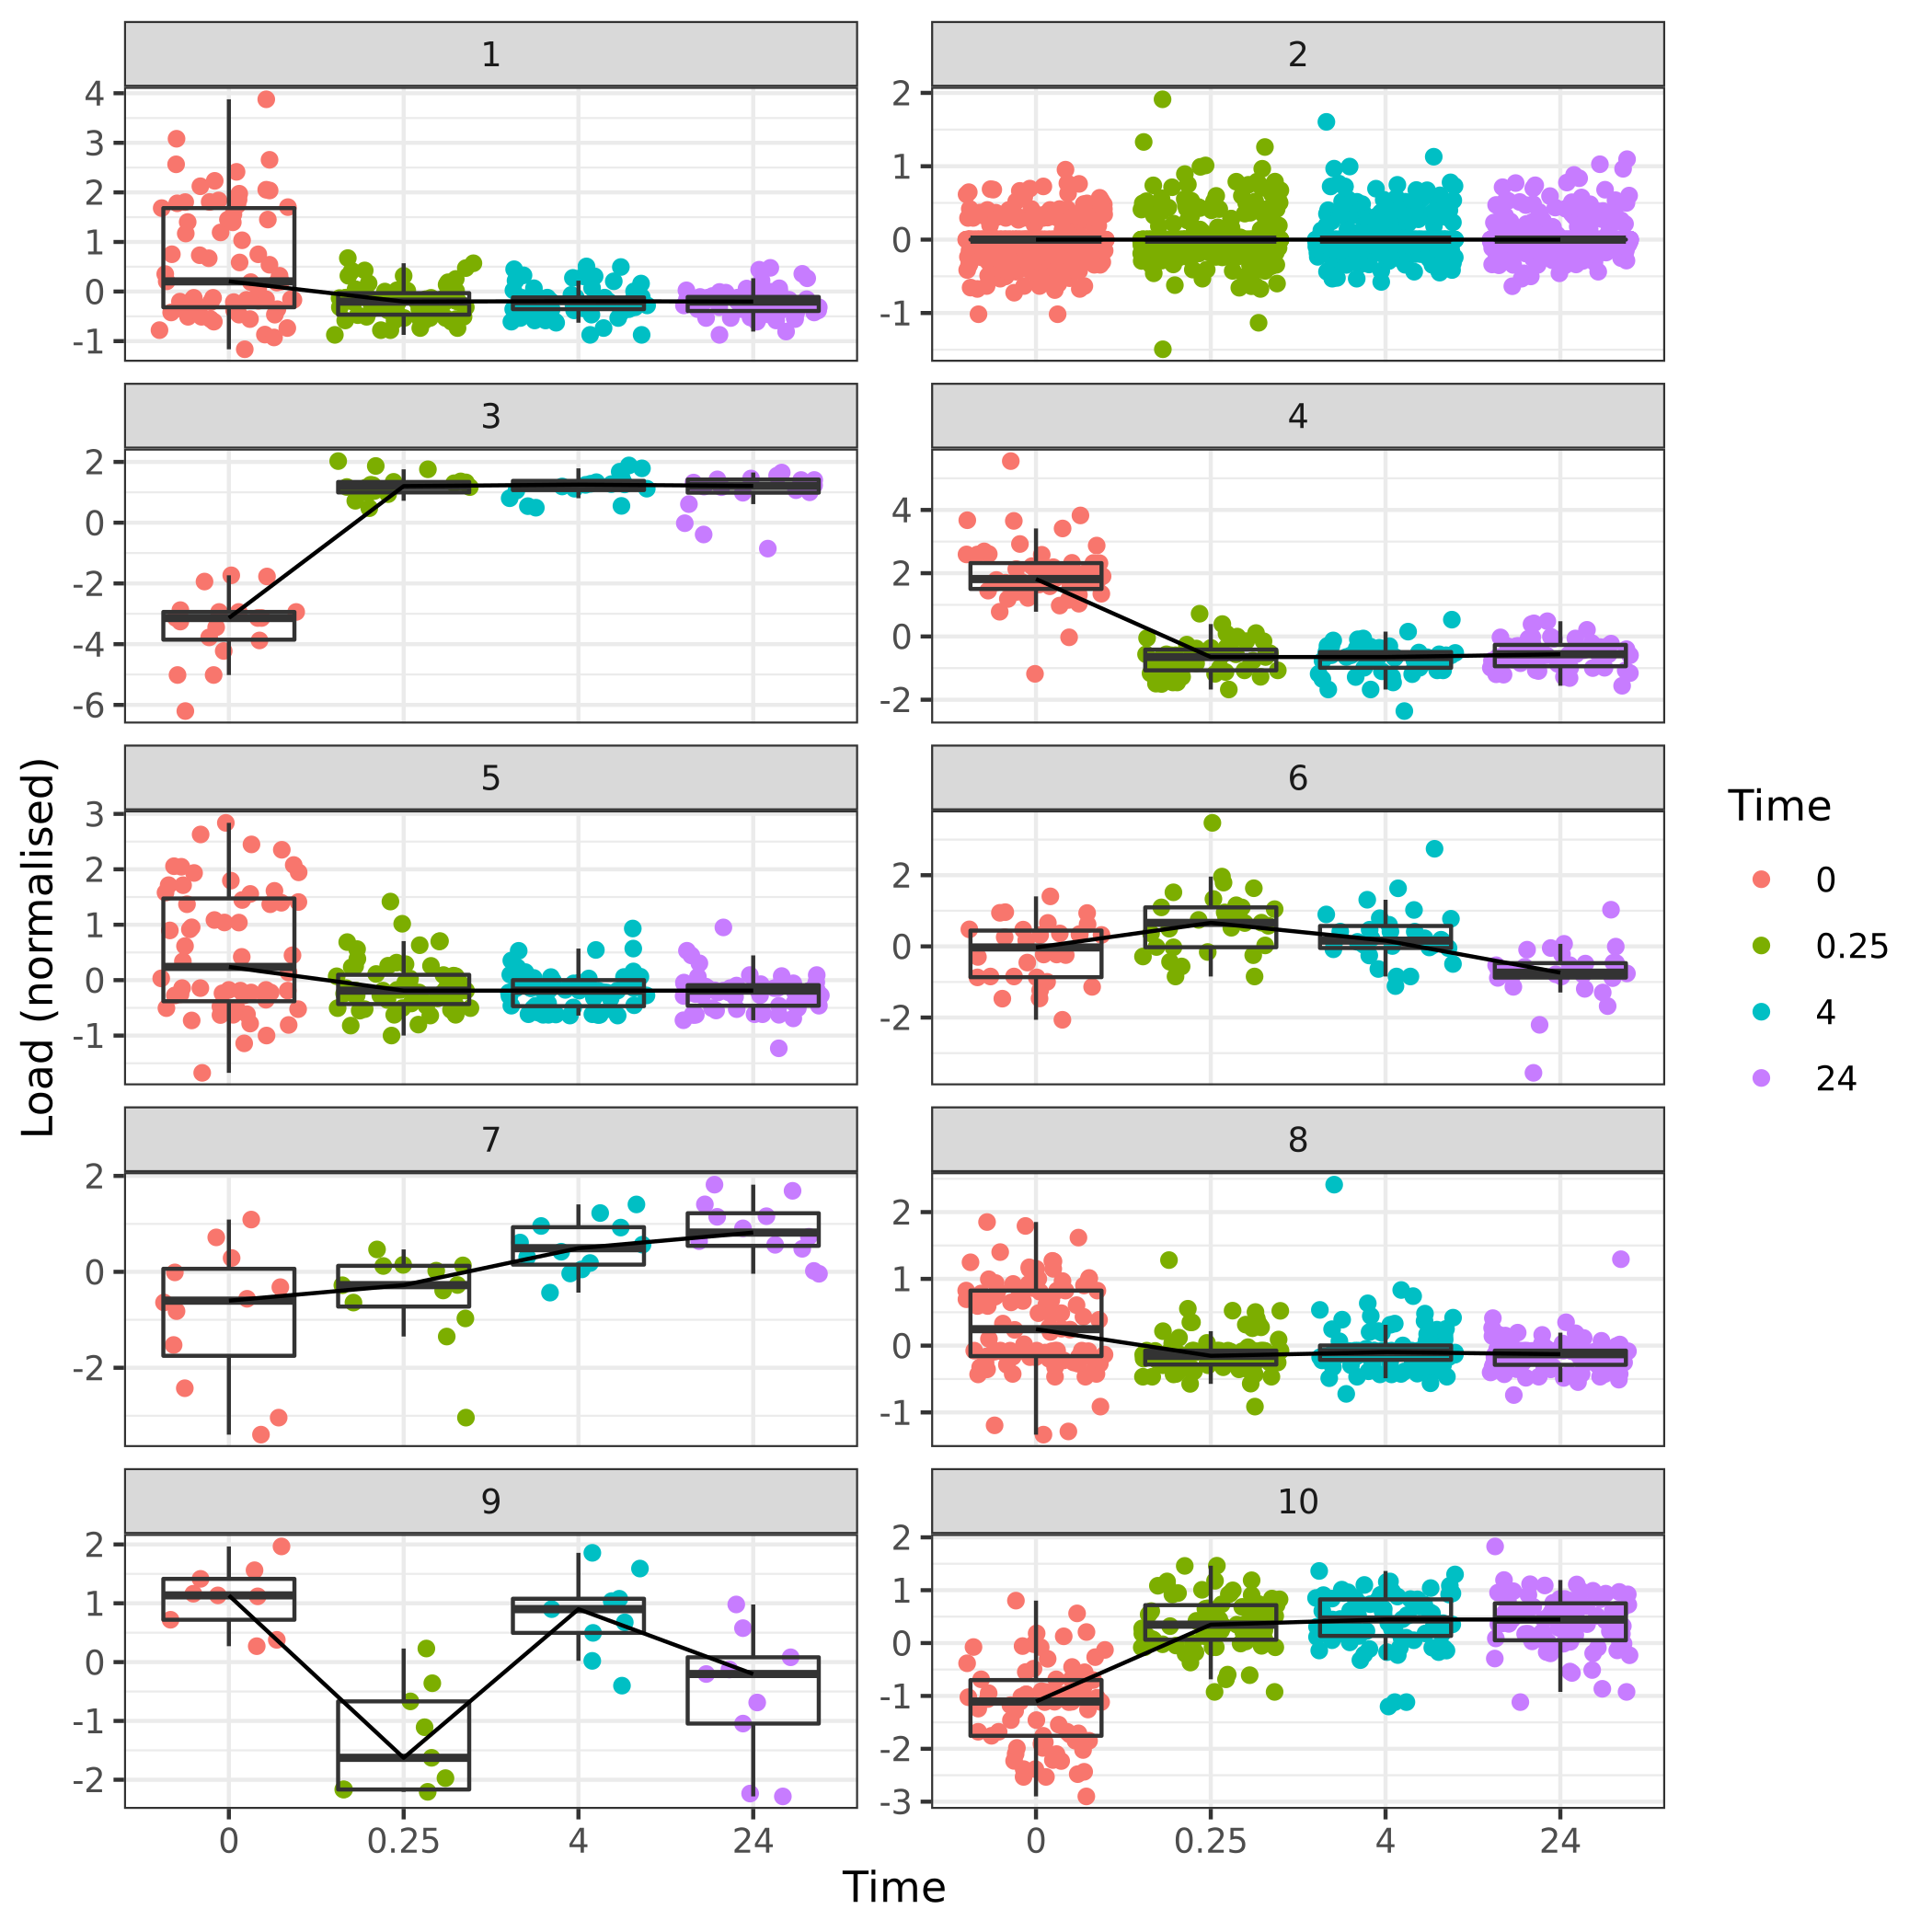
\includegraphics[width=.9\linewidth]{figure9/DEET/Legbox.png}
\end{center}
\subsubsection{PERM}
\label{sec:orgb02379f}
\begin{center}
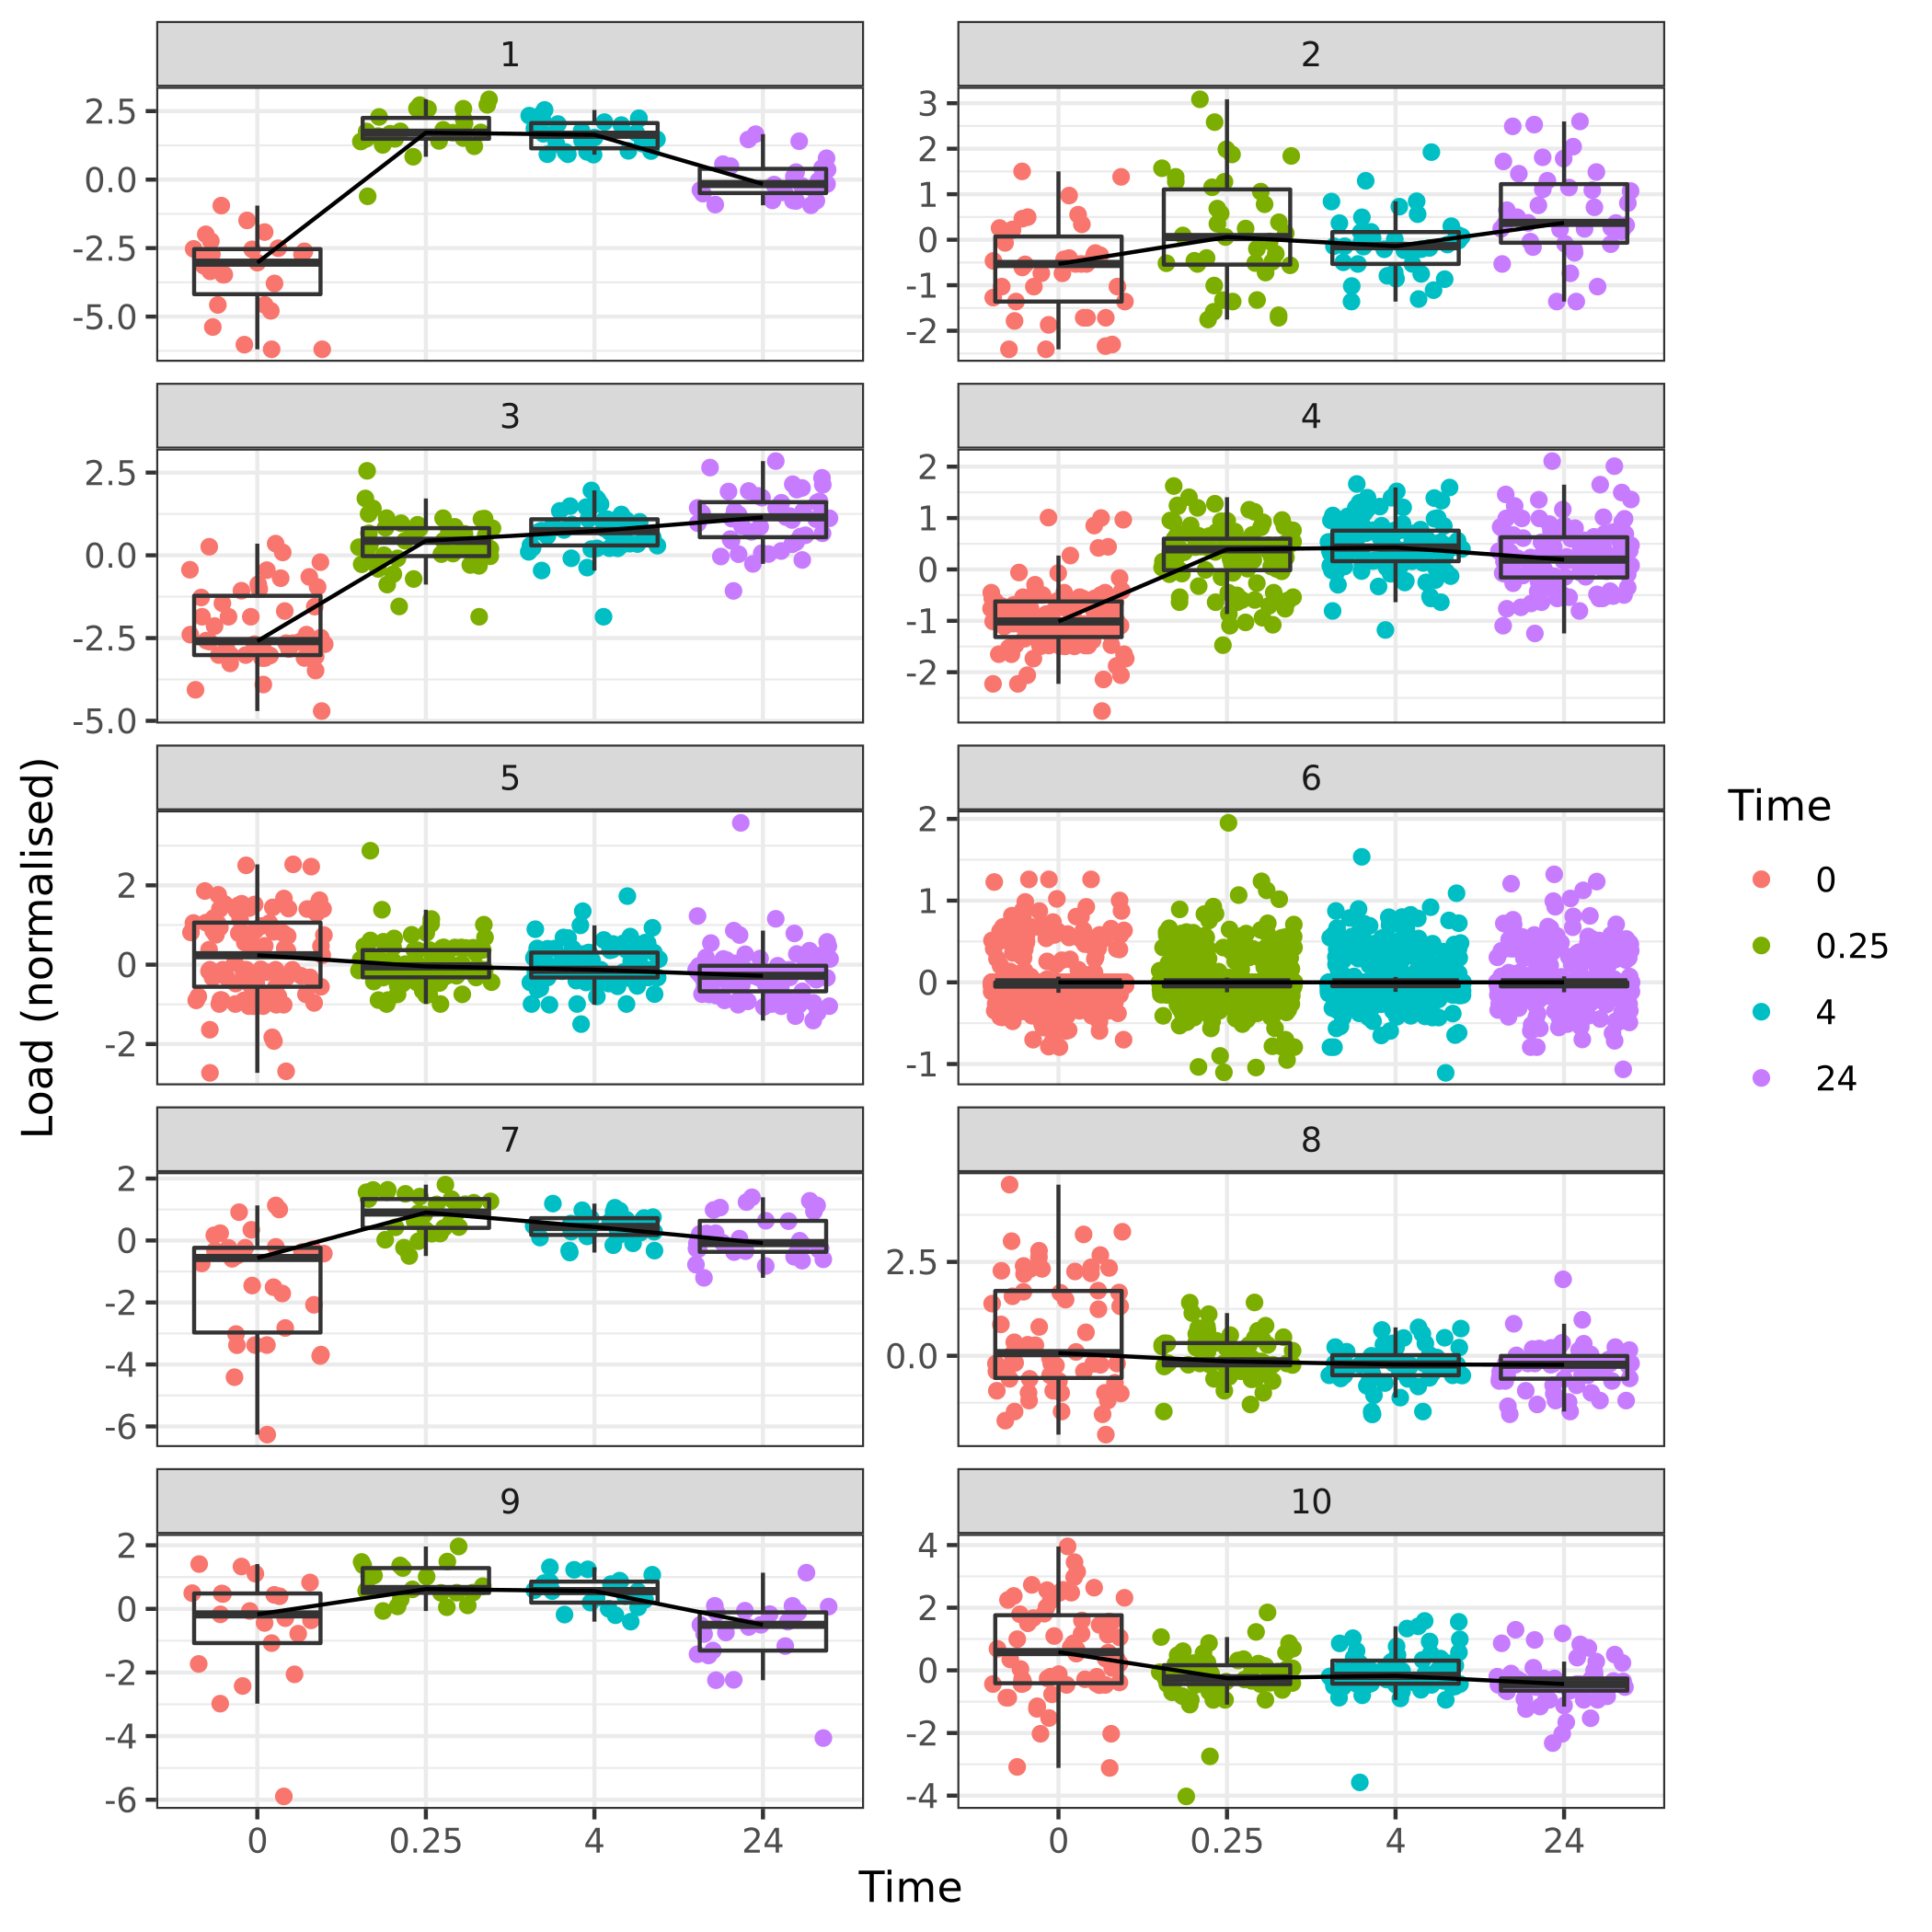
\includegraphics[width=.9\linewidth]{figure9/PERM/Legbox.png}
\end{center}
\subsubsection{Supplemental Tables}
\label{sec:orgcce9fb5}
\url{figure9/PERM/Legbox/cluster1.csv}
\subsection{Figure 10}
\label{sec:org7508fe2}
\subsubsection{DEET}
\label{sec:orgfaa377a}
\begin{center}
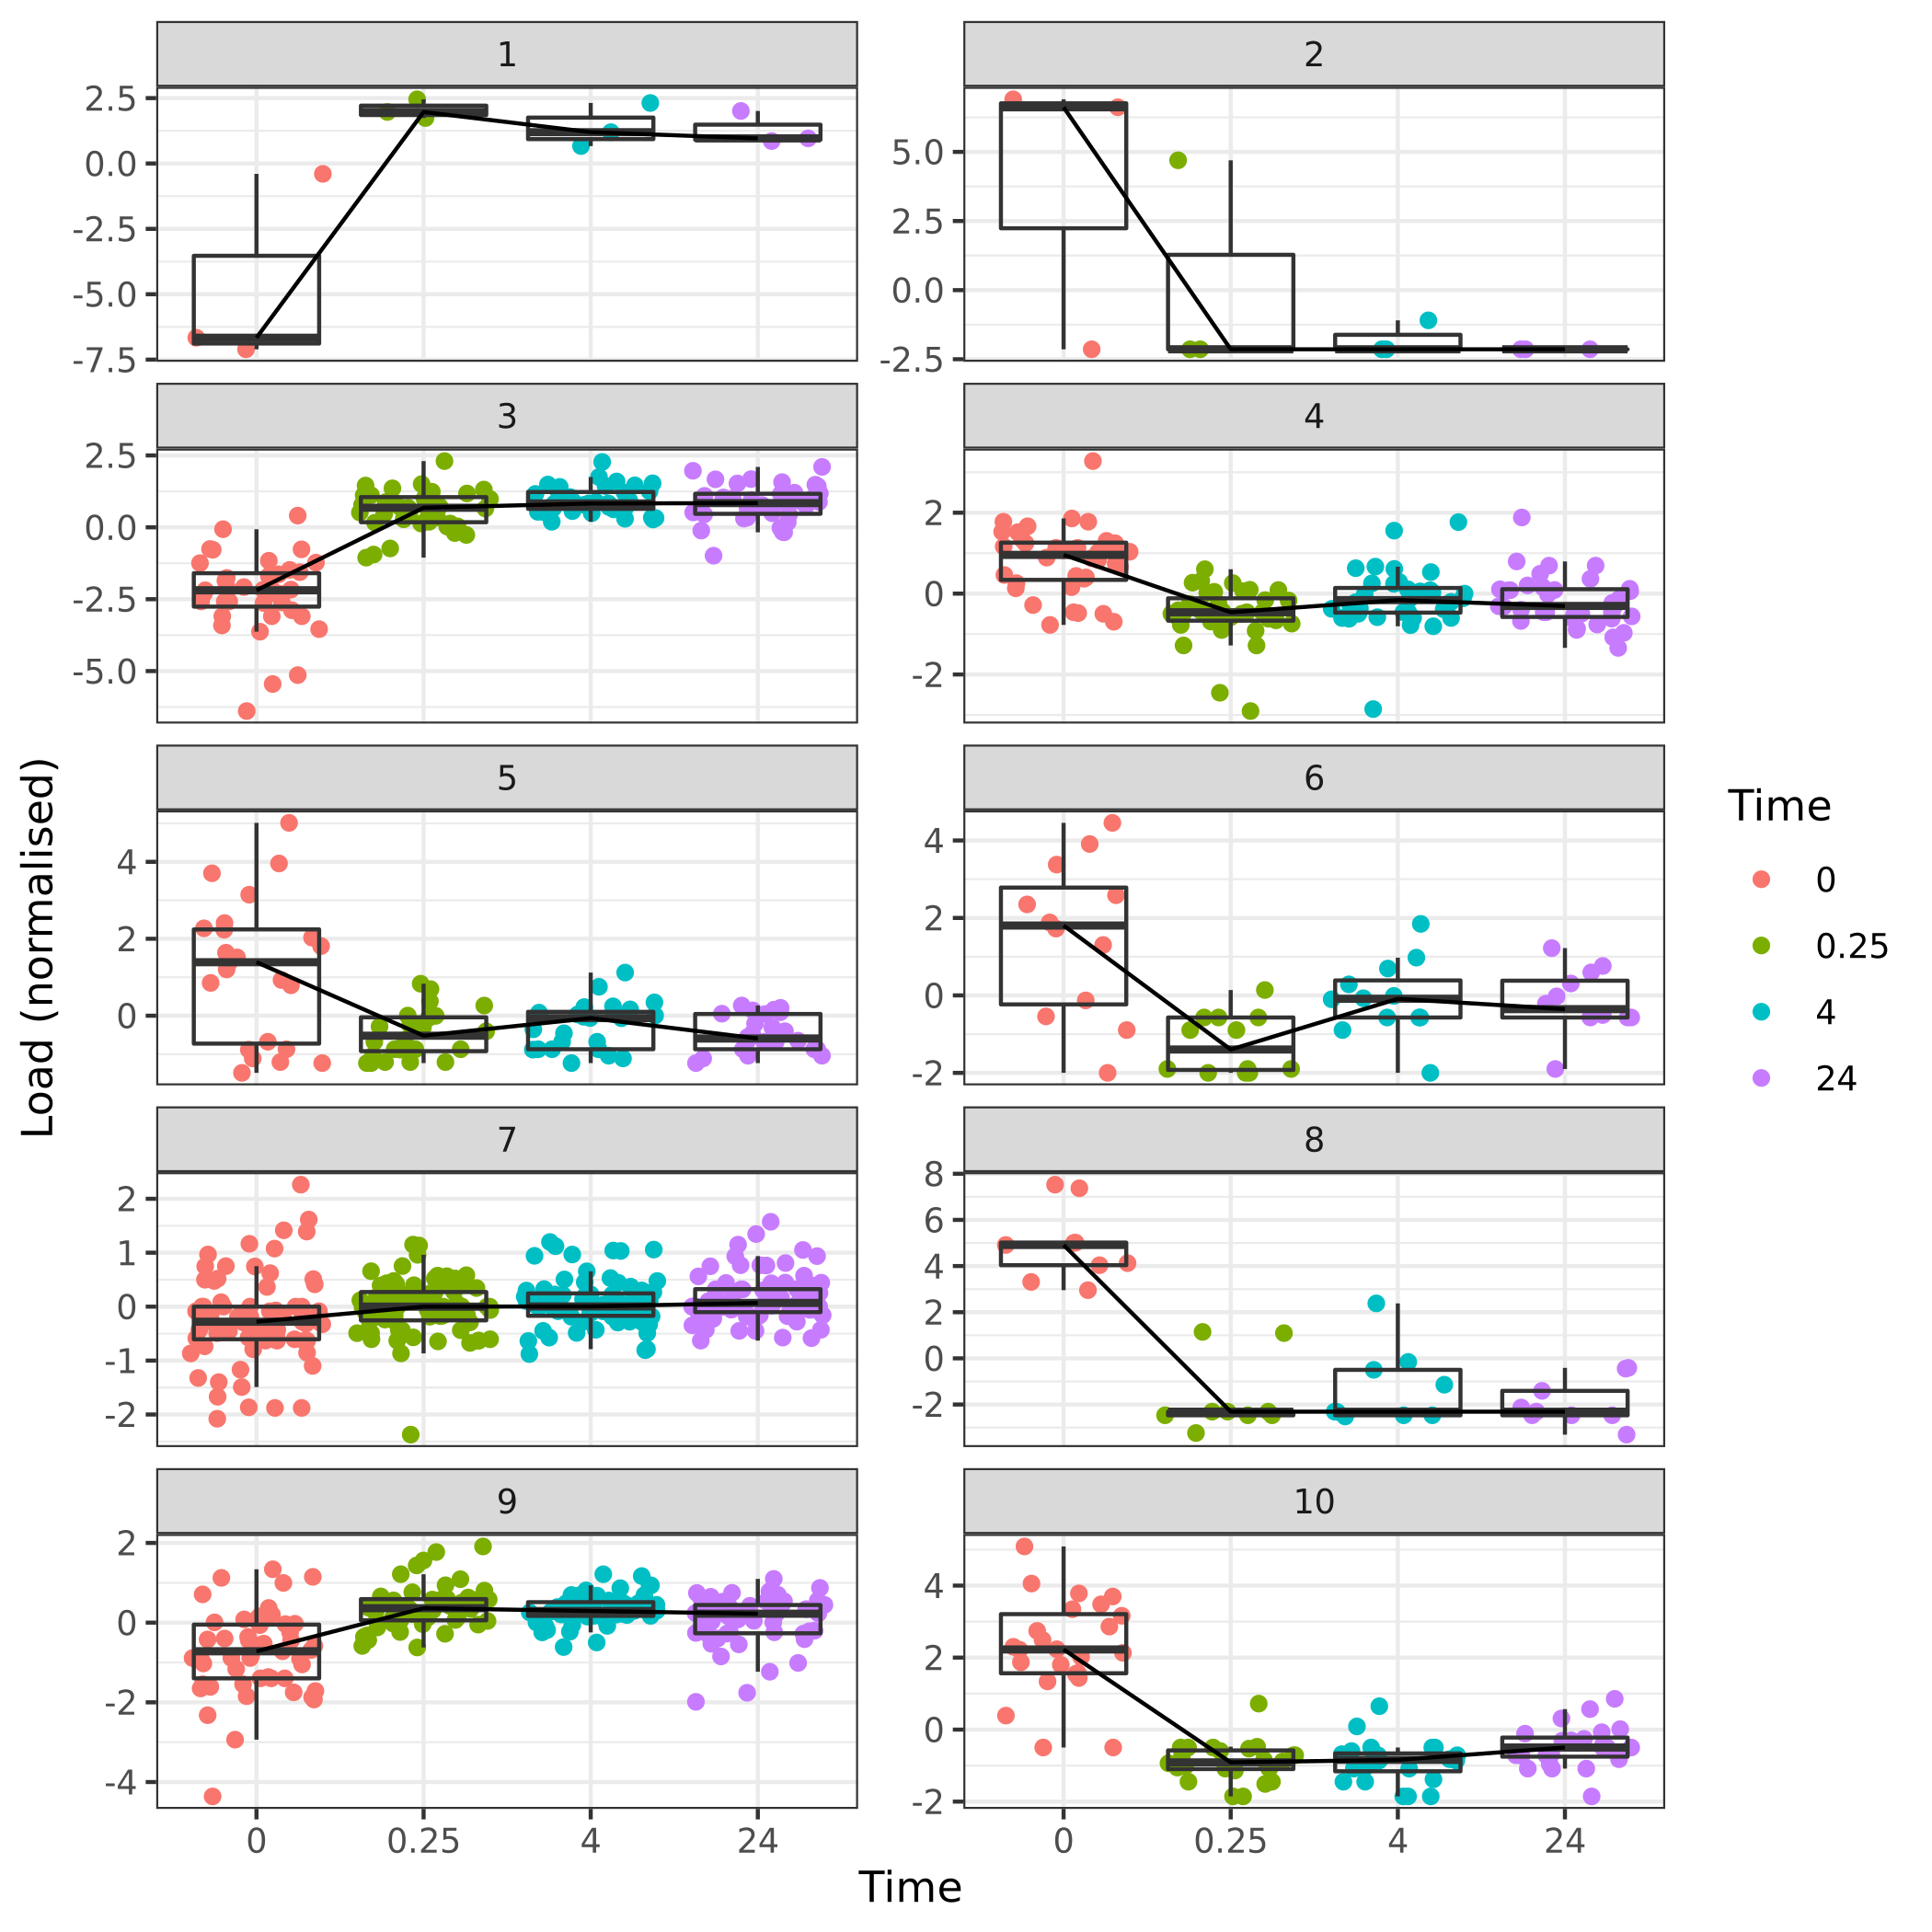
\includegraphics[width=.9\linewidth]{figure10/DEET/Bodybox.png}
\end{center}
\subsubsection{PERM}
\label{sec:org1667a82}
\begin{center}
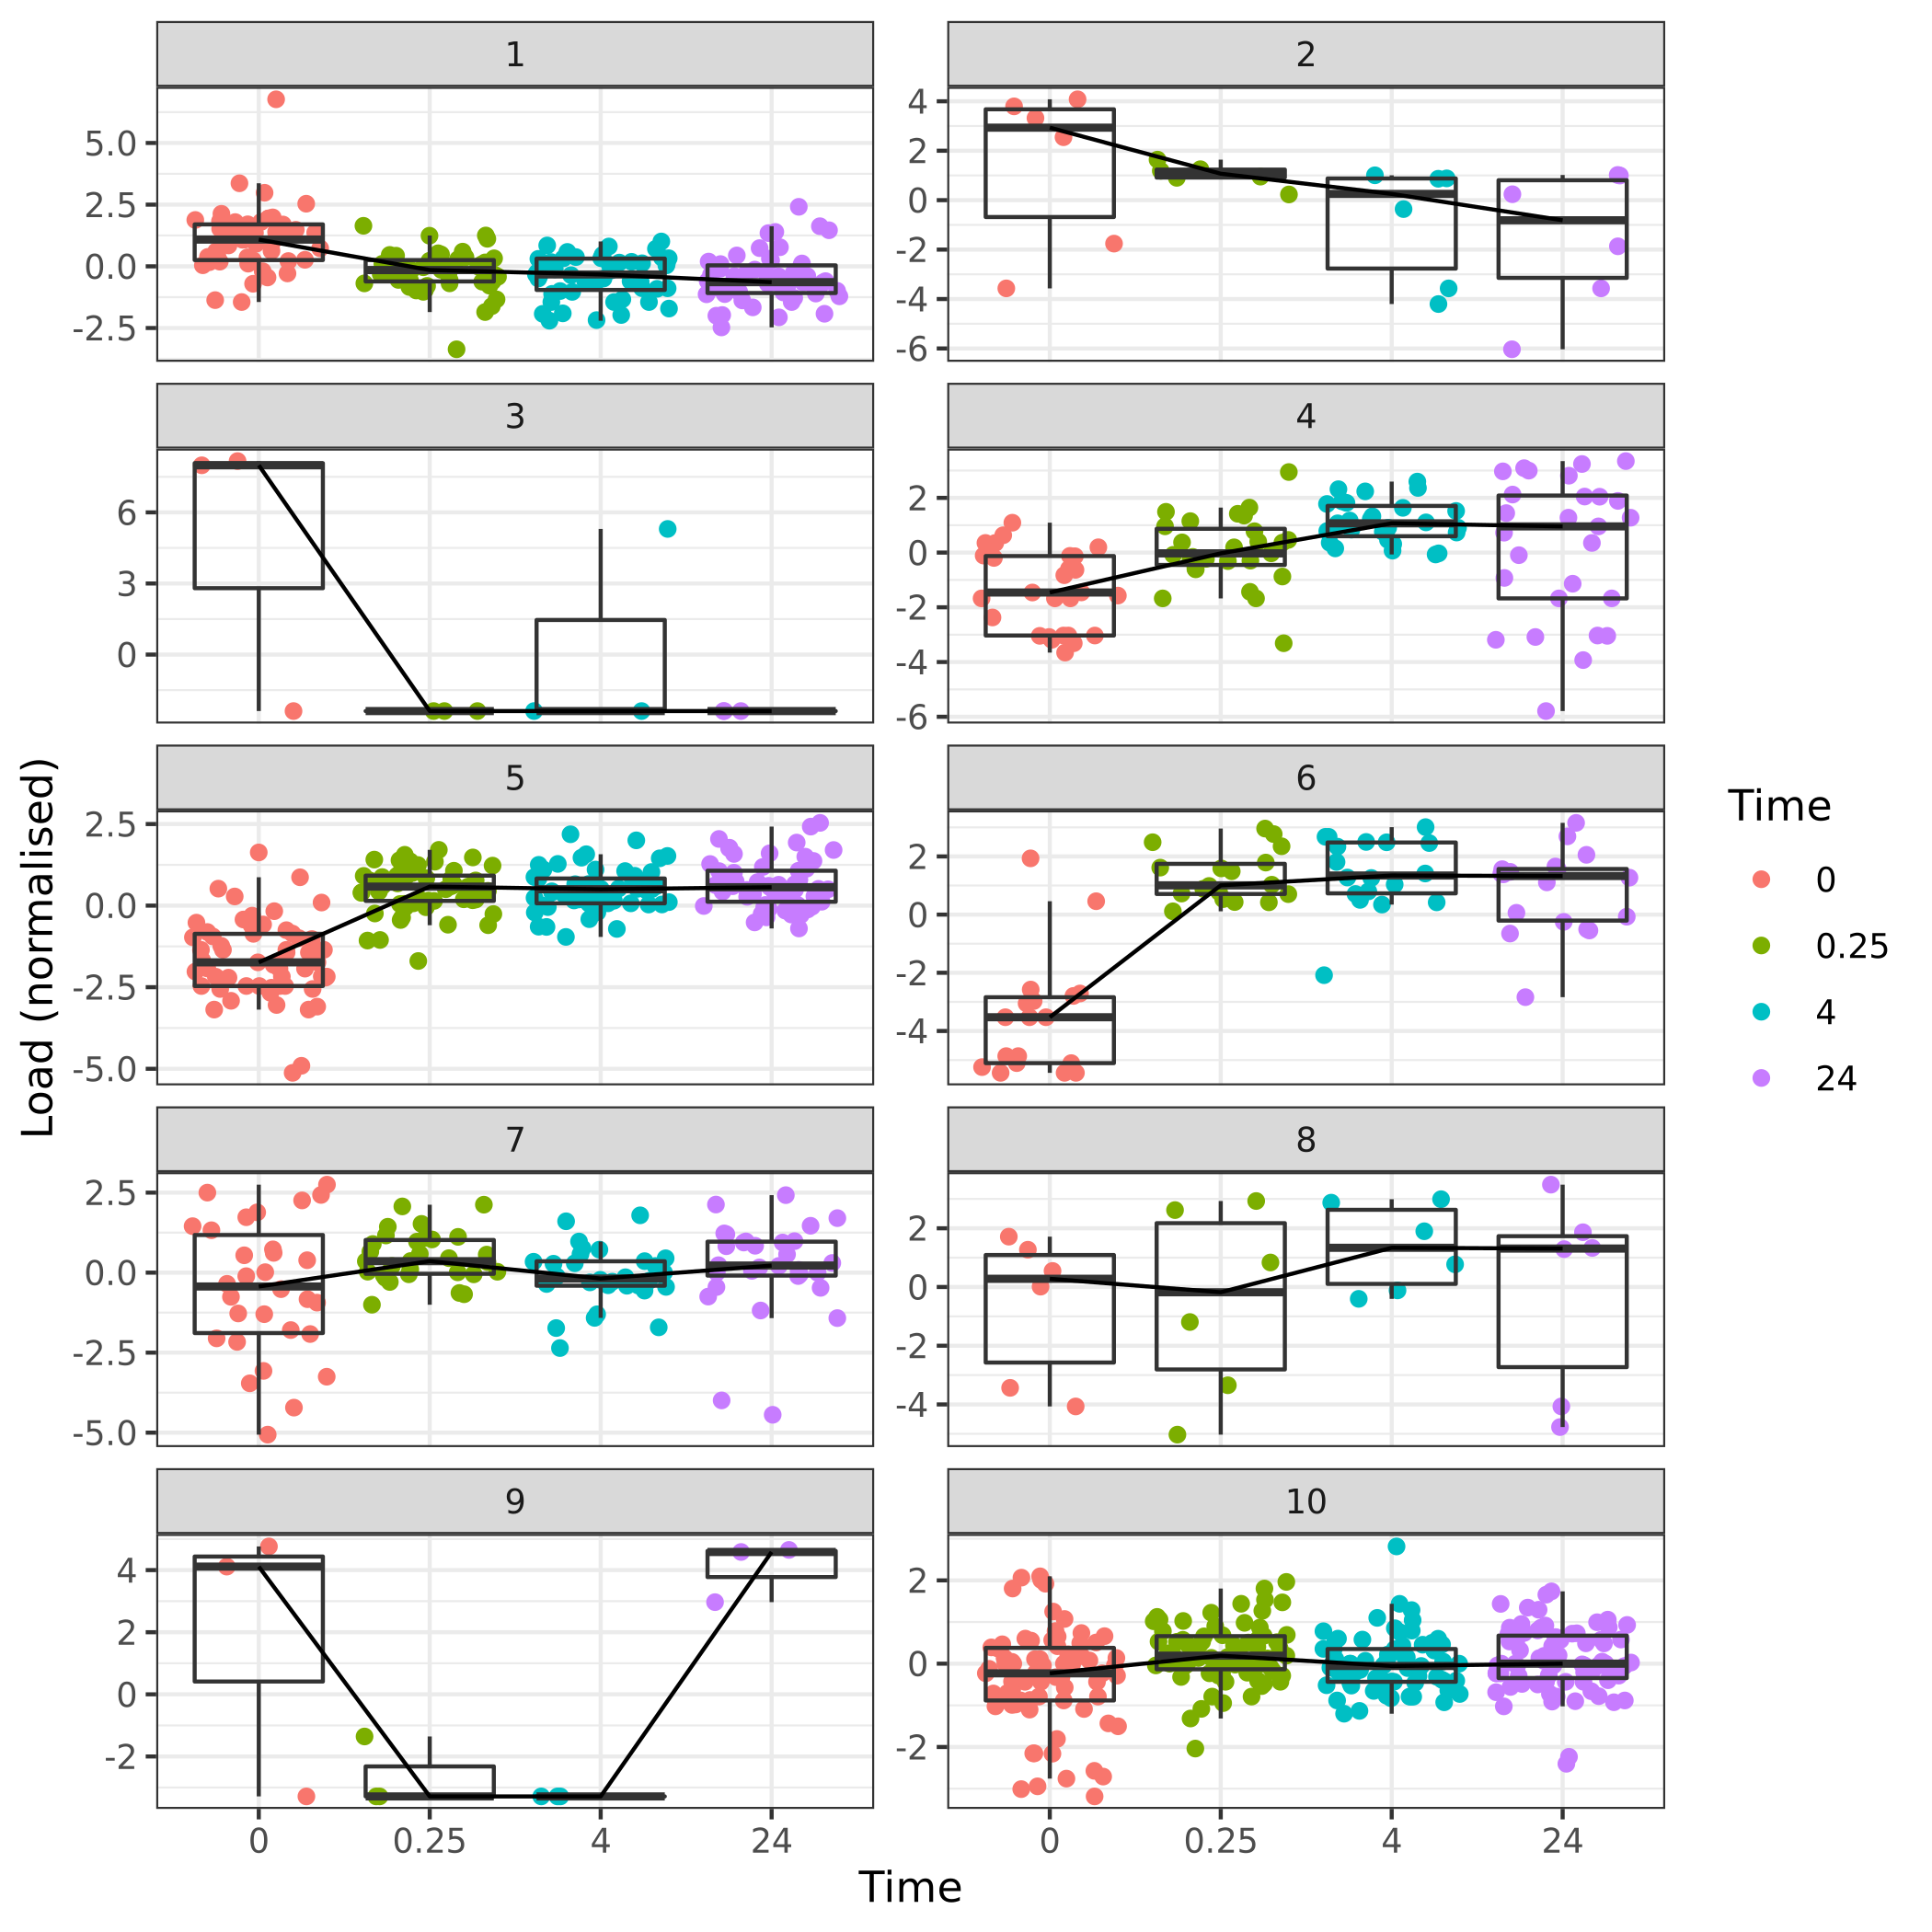
\includegraphics[width=.9\linewidth]{figure10/PERM/Bodybox.png}
\end{center}

\section{Discussion}
\label{sec:org9f24c09}
\end{document}
